\chapter{국소 보존 법칙에서 아인슈타인 장방정식까지}

아인슈타인 장방정식은 한 줄로 쓸 만큼 간단하지만, 성분별로 전개하면 악명 높을 만큼 다루기 어렵다. 계량에는 크리스토펠 기호가 많이 들어 있고, 크리스토펠 기호에는 계량의 미분이 들어 있으며, 곡률 텐서에는 크리스토펠 기호의 미분과 곱이 모두 들어 있다. 무엇을 풀어 보기도 전에 계산만으로 여러 페이지를 차지할 수 있다. 특정 계량을 다룰 때는 기호 계산 소프트웨어를 이용해 이런 계산을 정리하는 것이 대개 합리적이다.

원리는 계산보다 훨씬 간결하다. 따라서 방정식을 성분별로 하나씩 다루는 데서 시작하지는 않겠다. 중력이 어떤 형태의 방정식을 요구하는지 물어보자. 논의는 뉴턴 이론에서 시작해 국소 보존 법칙을 거쳐, 에너지와 운동량의 흐름 및 밀도와 일관되게 같아질 수 있는 곡률 텐서의 유일한 조합을 찾아내는 데 이른다. 이 장 전체에서 \(c=1\)를 사용한다.

\section{뉴턴 역학의 양방향 관계}

중력에는 서로 보완하는 두 가지 지침이 있다. 중력장은 물질이 어떻게 운동할지 알려 주고, 물질은 중력장이 어떤 상태일지 알려 준다. 이 양방향 관계는 뉴턴 역학에서도 이미 드러난다.

\(\phi(\mathbf{x},t)\)를 뉴턴 중력 퍼텐셜이라 하자. 질량이 \(m\)인 시험 물체가 받는 힘은
\begin{equation}
 \mathbf{F}=-m\nabla\phi.
\end{equation}
이다. 이를 \(\mathbf{F}=m\mathbf{a}\)와 결합하면 시험 질량이 소거되어
\begin{equation}
 \mathbf{a}=-\nabla\phi.
\end{equation}
를 얻는다. 이것이 양방향 관계의 첫 번째 방향이다. 장을 알면 질량과 무관하게 자유 낙하하는 모든 물체의 가속도를 알 수 있다.

반대 방향은 푸아송 방정식으로 주어진다.
\begin{equation}
 \nabla^2\phi=4\pi G\rho,
 \qquad
 \nabla^2=
 \frac{\partial^2}{\partial x^2}
 +\frac{\partial^2}{\partial y^2}
 +\frac{\partial^2}{\partial z^2},
 \label{eq:poisson}
\end{equation}
여기서 \(\rho(\mathbf{x},t)\)는 단위 부피당 질량이다. 인자 \(4\pi\)를 \(G\)의 정의에 넣을 수도 있지만, 그러면 다른 곳에 다시 나타날 뿐이다. 방정식~\eqref{eq:poisson}는 물질의 분포가 퍼텐셜의 원천임을 말해 준다.

총질량이 \(M\)인 구대칭 물체의 외부 해는
\begin{equation}
 \phi(r)=-\frac{GM}{r}.
 \label{eq:newton-potential}
\end{equation}
이다. 밀도는 중심 부근에 집중될 수도 있고, 균일하게 퍼져 있을 수도 있으며, 표면을 향해 점차 감소할 수도 있다. 외부 해에 반영되는 것은 구대칭성과 총질량뿐이다. 물질이 없는 곳에서는
\(\nabla^2\phi=0\)이고, \(1/r\)를 미분하면 역제곱 힘을 얻는다. 외부만 관심 대상이라면 원천을 점으로 줄여 그 점을 제외한 모든 곳에서 같은 식을 사용할 수 있다.

\begin{classroomqa}
\audiencequestion{구형 물체 내부의 밀도는 일정하다가 경계에서 불연속적으로 영이 되어야 하나요?}
\lecturerresponse{아닙니다. 이 논의에서는 구대칭이어야 하지만, 밀도가 일정할 필요도 없고 불연속적으로 변할 필요도 없습니다. 밀도는 영까지 부드럽게 감소할 수 있습니다. 내부의 그런 세부 사항은 총질량에만 의존하는 외부 퍼텐셜을 바꾸지 않습니다.
\lecturetimestamp{00:09:13--00:09:37}}
\end{classroomqa}

이 장의 기술은 멀리 떨어진 질량들 사이의 직접적인 힘보다 국소적인 형태를 띠지만, 뉴턴 중력에는 여전히 순간적인 원격 작용이 들어 있다. 원천을 움직이면 뉴턴 퍼텐셜은 모든 곳에서 동시에 변한다. 일반상대성이론은 힘 법칙뿐 아니라 이러한 순간적인 반응도 대체해야 한다.

\section{약한 장의 단서, 아직 방정식은 아니다}

첫 번째 지침의 상대론적 형태는 이미 알려져 있다. 시공간 계량이 주어지면 자유 낙하하는 입자는 시공간의 측지선을 따른다. 이제 물질이 계량을 결정하는 지침, 곧 푸아송 방정식의 상대론적 대체물이 필요하다.

슈바르츠실트 기하가 단서를 제공한다. 그 시간-시간 성분은
\begin{equation}
 g_{00}=1-\frac{2GM}{r}.
\end{equation}
이다. 방정식~\eqref{eq:newton-potential}을 사용하면 다음과 같이 된다.
\begin{equation}
 g_{00}=1+2\phi.
\end{equation}
따라서
\begin{equation}
 \nabla^2g_{00}=2\nabla^2\phi=8\pi G\rho.
 \label{eq:weak-mnemonic}
\end{equation}

방정식~\eqref{eq:weak-mnemonic}은 신중하게 받아들여야 한다. 이것은 아인슈타인 방정식이 아니라 기억을 돕는 식이다. 계량의 특정 성분과 비상대론적 원천을 사용한다. 그래도 우리가 찾는 식의 특징은 보여 준다. 한쪽에는 물질 밀도가, 다른 쪽에는 기하의 이계 미분이 놓인다. 푸아송 방정식에서 공변 장방정식으로 이어지는 대략적인 다리다.

이제 우변을 더 자세히 살펴보자. 상대론적 단위계에서는 질량이 에너지이므로, 우선 \(\rho\)를 에너지 밀도로 이해해야 한다. 하지만 에너지 밀도만으로는 완전한 상대론적 대상이 되지 않는다. 에너지 밀도와 함께 무엇이 필요한지 살펴보기 위해, 더 단순한 보존량부터 시작하자.

\section{전하 밀도, 전류, 국소 보존}

\(Q\)를 전하라 하고 \(\sigma\)를 전하 밀도라 하자.
\begin{equation}
 \sigma=\lim_{\Delta V\to0}\frac{\Delta Q}{\Delta V}.
\end{equation}
밀도는 한 시각에 작은 공간 부피 안에 전하가 얼마나 들어 있는지를 묻는다. 전류는 다른 질문을 한다. 공간에 무한소의 방향이 정해진 창을 놓고, 단위 면적과 단위 시간당 그 창을 통과하는 전하량을 센다. 가능한 세 방향에 따라 공간 전류의 성분 \(J^i\)가 정해진다.

차원을 비교하면 유익하다. 전하 밀도는 전하를 세 개의 공간 길이로 나눈 값이다. 전류는 전하를 두 개의 공간 길이와 하나의 시간 간격으로 나눈 값이다. \(c=1\)일 때 시간과 길이는 같은 단위를 가지므로 밀도와 전류의 차원은 일치한다. 이들은 다음과 같이 하나의 사차원 벡터를 이룬다.
\begin{equation}
 J^\mu=(J^0,J^1,J^2,J^3),
 \qquad J^0=\sigma.
\end{equation}

전하 보존은 우주 전체의 총전하가 변하지 않는다는 말에 그치지 않는다. 이는 국소적인 법칙이다. 전하가 강의실에서 사라졌다가 알파 센타우리에서 순간적으로 다시 나타날 수는 없다. 전하가 어떤 영역을 떠난다면 그 경계를 통과해야 한다. 작은 상자 안의 전하 감소량은 상자 벽을 통해 바깥으로 나가는 유량과 같다. 가우스 정리를 적용하면
\begin{equation}
 \dot{\sigma}+\nabla\cdot\mathbf{J}=0,
\end{equation}
을 얻고, 합산 규약을 사용하면
\begin{equation}
 \partial_\mu J^\mu=0.
 \label{eq:charge-continuity}
\end{equation}
이 된다. 곡선 좌표에서는 이에 대응하는 텐서 방정식을 공변 미분으로 쓴다.
\begin{equation}
 D_\mu J^\mu=0.
\end{equation}
공변 미분은 장식이 아니다. 이 미분을 사용해야 이 진술이 어떤 좌표계에서도 의미를 갖는다.

\section{에너지와 운동량에 두 지표가 필요한 이유}

전하 자체는 불변이다. 상대운동을 하는 관측자들은 전자의 전하량에는 동의하지만 전하 밀도나 전류에는 동의하지 않는다. 움직이는 관측자는 길이 수축된 부피를 관측할 수 있고, 다른 관측자에게 정지해 있는 전하가 흐르는 것을 볼 수도 있다. 따라서 총전하가 변하지 않더라도 기준계가 바뀌면 밀도와 전류는 서로 섞인다.

에너지와 운동량은 더 복잡하다. 이들의 총량조차 기준계에 따라 달라진다. 한 관측자에게는 입자가 정지해 있어 정지 에너지만 지니고 공간 운동량은 없다. 그 옆을 지나가는 다른 관측자에게는 운동 에너지와 운동량이 모두 보인다. 이 네 물리량은 다음 운동량 사차원 벡터를 이룬다.
\begin{equation}
 P^\nu=(P^0,P^1,P^2,P^3),
 \qquad P^0=E.
\end{equation}
각 성분 \(P^\nu\)은 국소적으로 보존된다. 따라서 각각 밀도와 흐름을 가진다. 한 지표는 보존되는 물리량을 나타내고, 다른 지표는 밀도인지 흐름 방향인지를 나타낸다.

에너지부터 살펴보자. 에너지 밀도는 \(T^{00}\)이다. 에너지는 창을 통과할 수도 있으므로, \(T^{0i}\)는 \(x^i\) 방향의 에너지 흐름이다. 이제 운동량의 \(i\) 성분을 보자. 그 밀도는 \(T^{i0}\)이고 \(x^j\) 방향의 흐름은 \(T^{ij}\)이다. 이 규약에서는 다음과 같다.
\begin{itemize}
 \item \(T^{00}\)는 에너지 밀도,
 \item \(T^{0i}\)는 \(i\) 방향의 에너지 유량,
 \item \(T^{i0}\)는 운동량의 \(i\) 성분 밀도,
 \item \(T^{ij}\)는 \(i\) 운동량이 \(j\)에 수직인 면을 통과하는 유량이다.
\end{itemize}
공간 블록 \(T^{ij}\)는 나중에 응력으로 확인할 수 있다. 대각 성분에는 압력이 포함되고, 비대각 성분은 전단을 나타낸다.

\begin{classroomqa}
\audiencequestion{\(T^{m0}(x)\)를 운동량의 \(m\) 성분 밀도라고 할 때, \(x\) 자체가 위치의 \(m\) 성분을 뜻하나요?}
\lecturerresponse{아닙니다. 인자 \(x\)는 밀도가 평가되는 시공간 위치를 나타내며, 모든 좌표를 뜻합니다. 지표 \(m\)는 어떤 운동량 성분을 세는지를 표시합니다.
\lecturetimestamp{00:41:07--00:41:27}}
\end{classroomqa}

\(\nu\)를 고정할 때마다 국소 보존 법칙은 연속 방정식을 준다.
\begin{equation}
 D_\mu T^{\nu\mu}=0.
 \label{eq:stress-continuity}
\end{equation}
\(\nu\)의 네 값은 에너지에 관한 방정식 하나와 운동량에 관한 방정식 세 개를 준다. 이 밀도와 흐름을 함께 모으면 에너지-운동량 텐서가 된다.

\begin{figure}[htbp]
\centering
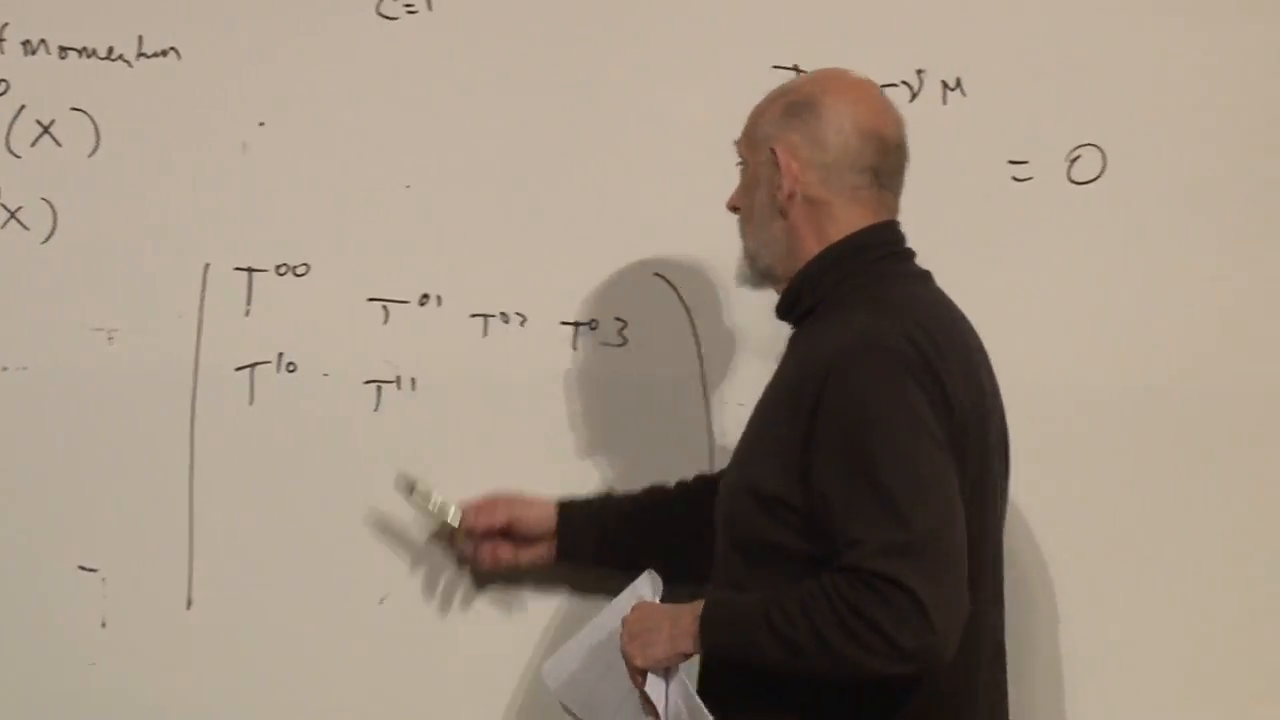
\includegraphics[width=0.84\textwidth]{lecture_09_figure_02.png}
\caption{칠판에 그려 가는 에너지-운동량 배열. 첫 번째 지표는 에너지 또는 운동량 성분을 선택하고, 두 번째 지표는 밀도 또는 흐름을 선택한다.}
\lectureframe{00:44:30}
\end{figure}

전체 배열은 다음과 같다.
\begin{equation}
 T^{\mu\nu}=
 \begin{pmatrix}
 T^{00}&T^{01}&T^{02}&T^{03}\\
 T^{10}&T^{11}&T^{12}&T^{13}\\
 T^{20}&T^{21}&T^{22}&T^{23}\\
 T^{30}&T^{31}&T^{32}&T^{33}
 \end{pmatrix}.
\end{equation}
상대론적 역학과 장 이론의 또 다른 정리에 따르면 중력과 관련된 응력-에너지 텐서는 대칭이다.
\begin{equation}
 T^{\mu\nu}=T^{\nu\mu}.
 \label{eq:stress-symmetry}
\end{equation}
특히 에너지 유량과 운동량 밀도는 서로 대응하는 비대각 성분을 반대쪽에서 본 것이다. 대칭성 덕분에 방정식~\eqref{eq:stress-continuity}을 익숙한 형태로 쓸 수도 있다.
\begin{equation}
 D_\mu T^{\mu\nu}=0.
 \label{eq:stress-conservation}
\end{equation}

\begin{classroomqa}
\audiencequestion{전하 전류에는 지표가 하나만 필요했는데 에너지-운동량에는 왜 지표가 하나 더 붙었나요?}
\lecturerresponse{전류의 지표 하나가 이미 밀도와 흐름 방향을 구별합니다. 보존되는 전하가 스칼라이므로 전하에는 별도의 표지가 필요하지 않습니다. 에너지와 세 운동량은 그 자체로 사차원 성분이므로 첫 번째 지표는 어떤 보존량인지를, 두 번째 지표는 밀도인지 흐름인지를 나타냅니다.
\lecturetimestamp{00:45:31--00:47:24}}
\end{classroomqa}

\begin{classroomqa}
\audiencequestion{\(T^{\mu\nu}\) 행렬 전체가 대칭인가요, 아니면 에너지 유량과 운동량 밀도에 해당하는 성분만 대칭인가요?}
\lecturerresponse{행렬 전체가 대칭입니다. 압력과 응력을 포함한 공간 성분의 자세한 의미는 뒤에서 다루겠습니다.
\lecturetimestamp{00:47:32--00:47:54}}
\end{classroomqa}

따라서 에너지 밀도는 더 큰 대상의 한 부분에 불과했다. 중력의 원천이 일관되게 \(T^{00}\)만일 수는 없다. 전체 텐서가 관련되어야 한다.

\section{법칙은 한 성분만을 선택할 수 없다}

곡률을 계산하지 않고도 텐서 방정식이 필요한 이유를 알 수 있다. \(A_i\)와 \(B_i\)가 벡터이고, 제안된 법칙이 \(A_3=B_3\)뿐이라고 하자. 이 등식이 모든 회전된 기준계에서도 성립해야 한다면 세 번째 축을 두 번째 축으로 회전하자. 같은 법칙은 이제 \(A_2=B_2\)이라고 말하며, 또 다른 회전은 \(A_1=B_1\)을 요구한다. 기준계에 무관한 법칙은 실은 벡터 방정식
\begin{equation}
 A_i=B_i.
\end{equation}
이다.

로런츠 변환은 같은 논리를 시간 성분에도 적용한다. \(A^0=B^0\)이 모든 관성계에서 성립해야 한다면 로런츠 부스트가 시간 성분과 공간 성분을 섞으므로 완전한 방정식 \(A^\mu=B^\mu\)이 따라야 한다. 올바른 상대론적 법칙은 같은 종류의 텐서끼리 등식으로 연결해야 한다.

뉴턴식 기억 보조 식은 \(T^{00}\)만을 선택했지만, 상대론적 방정식은 다음 형태여야 한다.
\begin{equation}
 G_{\mu\nu}=8\pi G\,T_{\mu\nu},
 \label{eq:field-schematic}
\end{equation}
여기서 기호 \(G_{\mu\nu}\)는 우선 자리표시자일 뿐이다. 필요한 성질은 이제 분명하다.
\begin{enumerate}
 \item 대칭인 이계 텐서여야 한다.
 \item 물질이 아니라 계량으로 구성되어야 한다.
 \item 계량의 이계 미분을 포함해야 한다.
 \item 공변 발산이 영이어야 한다.
\end{enumerate}
마지막 조건은 방정식~\eqref{eq:stress-conservation}에서 따라온다.

\section{곡률 텐서 가운데서 찾기}

크리스토펠 기호에는 계량의 일계 미분이 들어 있다.
\begin{equation}
 \Gamma^\sigma_{\tau\nu}
 =
 \frac12 g^{\sigma\delta}
 \left(
 \partial_\tau g_{\delta\nu}
 +\partial_\nu g_{\delta\tau}
 -\partial_\delta g_{\tau\nu}
 \right).
 \label{eq:christoffel}
\end{equation}
크리스토펠 기호는 텐서가 아니므로, 그 자체로는 좌변을 구성할 수 없다. 리만 곡률 텐서는 텐서다.
\begin{equation}
 R^\rho{}_{\sigma\mu\nu}
 =
 \partial_\mu\Gamma^\rho_{\nu\sigma}
 -\partial_\nu\Gamma^\rho_{\mu\sigma}
 +\Gamma^\rho_{\mu\lambda}\Gamma^\lambda_{\nu\sigma}
 -\Gamma^\rho_{\nu\lambda}\Gamma^\lambda_{\mu\sigma}.
 \label{eq:riemann}
\end{equation}
처음 두 항에는 계량의 이계 미분이 들어 있고, 마지막 두 항에는 일계 미분의 곱이 들어 있다. 이는 뉴턴 방정식이 시사하는 미분 차수와 정확히 일치한다.

문제는 지표 구조다. \(R^\rho{}_{\sigma\mu\nu}\)에는 지표가 네 개 있지만 \(T_{\mu\nu}\)에는 두 개뿐이다. 적절한 반변 지표와 공변 지표를 축약하면 리치 텐서
\begin{equation}
 R_{\mu\nu}=R^\lambda{}_{\mu\lambda\nu}.
 \label{eq:ricci}
\end{equation}
를 얻는다. 다른 겉보기 축약은 리만 텐서의 대칭성 때문에 영이 되거나, 부호와 지표 규약만 다른 같은 대상을 준다. 리치 텐서는 대칭이지만 전체 리만 텐서보다 정보가 적다. 리만 텐서는 영이 아니어도 리치 텐서는 영일 수 있다.

\begin{classroomqa}
\audiencequestion{리만 텐서의 아래 지표 두 개를 바로 축약할 수 있나요? 축약하려면 공변 지표 하나와 반변 지표 하나가 필요하지 않나요?}
\lecturerresponse{맞습니다. 역계량으로 지표 하나를 먼저 올려야 합니다. 또는 축약에 \(g^{\mu\nu}\)를 포함하면 됩니다. \(R^\lambda{}_{\mu\lambda\nu}\)로 쓰면 필요한 반변-공변 지표 쌍이 명시됩니다.
\lecturetimestamp{01:00:09--01:00:33}}
\end{classroomqa}

리치 텐서를 다시 축약하면 곡률 스칼라
\begin{equation}
 R=g^{\mu\nu}R_{\mu\nu}.
 \label{eq:ricci-scalar}
\end{equation}
를 얻는다. 이 스칼라에 \(g_{\mu\nu}\)를 곱하면 또 하나의 대칭 이계 텐서가 된다. 따라서 자연스러운 후보 두 가지를 찾았다.
\begin{equation}
 R_{\mu\nu},
 \qquad
 g_{\mu\nu}R.
\end{equation}

\begin{figure}[htbp]
\centering
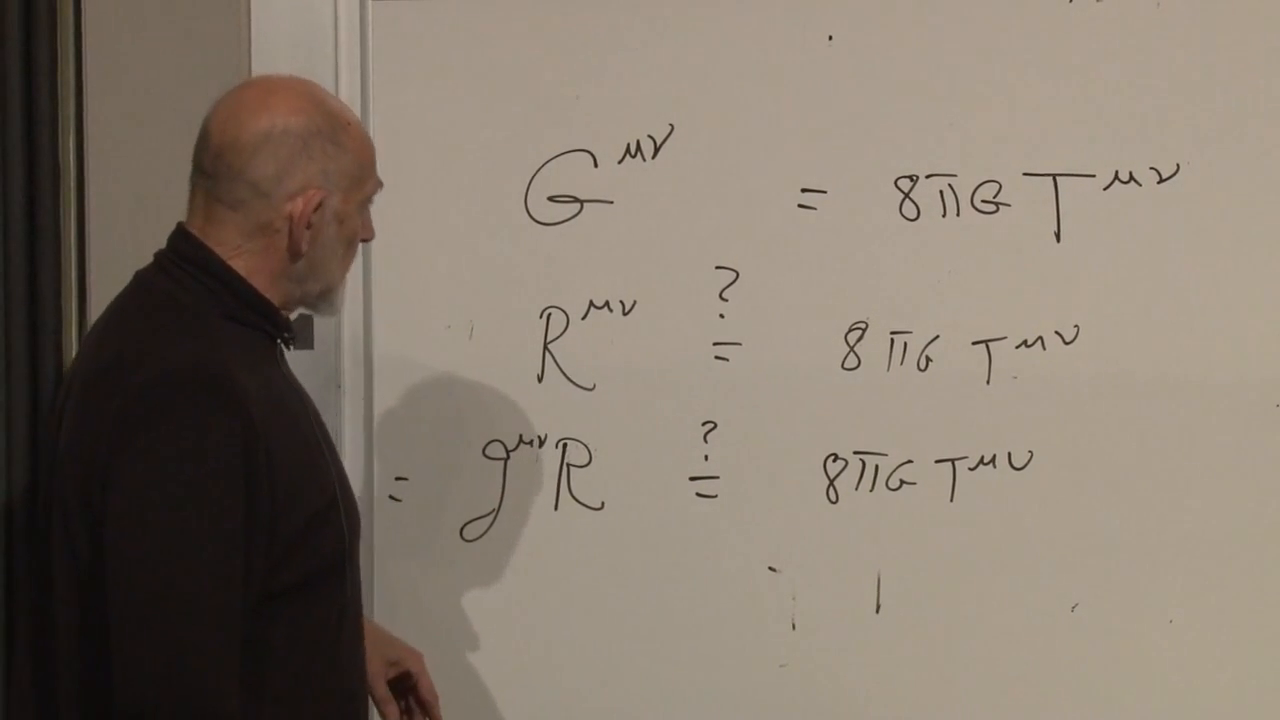
\includegraphics[width=0.78\textwidth]{lecture_09_figure_03.png}
\caption{칠판에 적은 기하학적 텐서 후보 두 가지. 이 단계에서는 둘 다 올바른 계수와 미분 차수를 가지므로 각각 물음표가 붙어 있다.}
\lectureframe{01:04:56}
\end{figure}

검토 중인 후보는 다음과 같다.
\begin{align}
 R_{\mu\nu}&\stackrel{?}{=}8\pi G\,T_{\mu\nu},\\
 g_{\mu\nu}R&\stackrel{?}{=}8\pi G\,T_{\mu\nu}.
\end{align}
지표가 맞는다는 이유만으로 어느 쪽도 받아들일 수는 없다. 보존 법칙으로 검증해야 한다.

\section{발산 검증}

방정식~\eqref{eq:field-schematic}이 옳다면 다음 식이
\begin{equation}
 D_\mu G^{\mu\nu}=0
\end{equation}
항등적으로 성립해야 한다. \(D_\mu T^{\mu\nu}=0\)이기 때문이다. 곡률 스칼라 후보부터 살펴보자. 곱의 미분 법칙을 적용하면
\begin{equation}
 D_\mu\!\left(g^{\mu\nu}R\right)
 =
 \left(D_\mu g^{\mu\nu}\right)R
 +g^{\mu\nu}D_\mu R.
 \label{eq:product-rule}
\end{equation}

\begin{figure}[htbp]
\centering
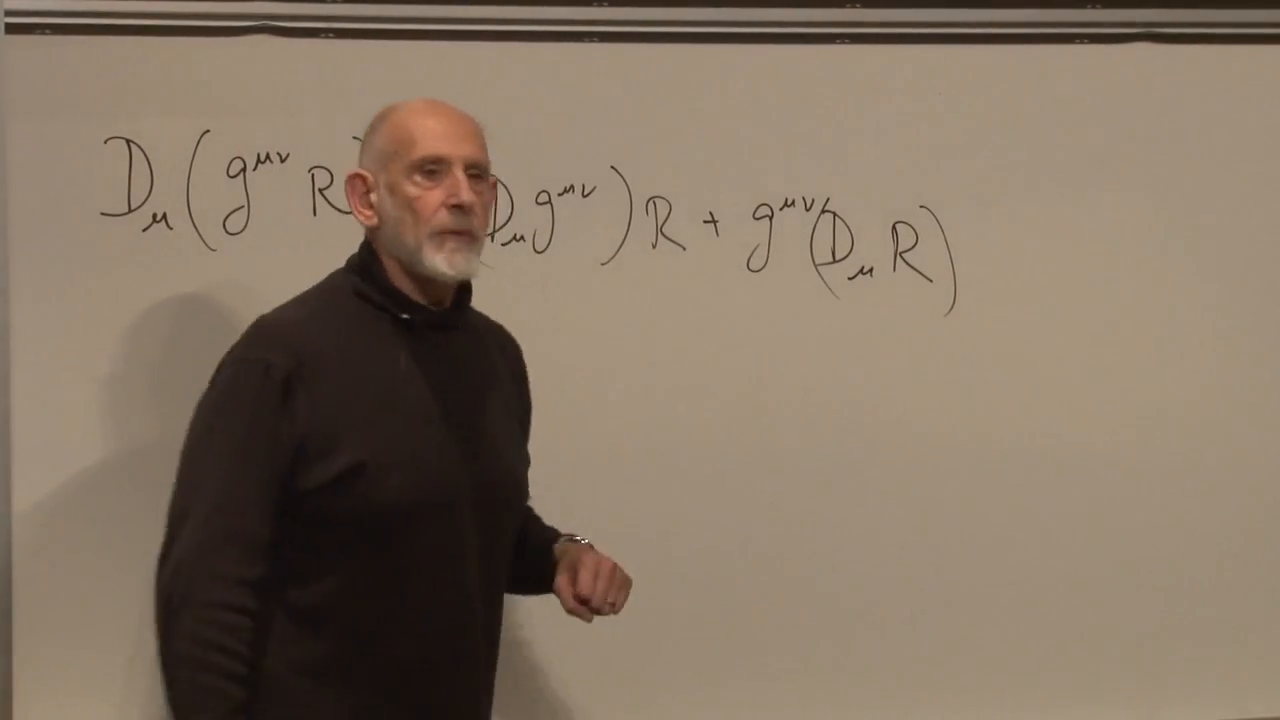
\includegraphics[width=0.84\textwidth]{lecture_09_figure_04.png}
\caption{\(D_\mu(g^{\mu\nu}R)\)에 공변 곱의 미분 법칙을 적용한다.}
\lectureframe{01:07:12}
\end{figure}

계량 호환성은
\begin{equation}
 D_\mu g^{\alpha\beta}=0.
 \label{eq:metric-compatibility}
\end{equation}
을 뜻한다. 이는 에너지-운동량 보존에서 나오는 결과가 아니라 레비치비타 접속의 독립적인 기하학적 성질이다. \(R\)는 스칼라이므로 \(D_\mu R=\partial_\mu R\)이다. 따라서 방정식~\eqref{eq:product-rule}은 다음과 같이 된다.
\begin{equation}
 D_\mu(g^{\mu\nu}R)
 =g^{\mu\nu}\partial_\mu R
 =D^\nu R,
\end{equation}
이는 일반적으로 영이 아니다. 그러므로 후보 \(g^{\mu\nu}R\)는 탈락한다.

리치 텐서의 경우에 해당하는 계산은 조금 더 길다. 그 결과는 축약된 비앙키 항등식이다.
\begin{equation}
 D_\mu R^{\mu\nu}=\frac12 D^\nu R.
 \label{eq:contracted-bianchi}
\end{equation}
따라서 \(R^{\mu\nu}\)도 단독으로는 성립하지 않는다. 하지만 두 후보의 발산은 정확히 상쇄에 필요한 비율을 가진다.
\begin{equation}
 D_\mu\left(
 R^{\mu\nu}-\frac12 g^{\mu\nu}R
 \right)=0.
\end{equation}
이로부터 아인슈타인 텐서
\begin{equation}
 \boxed{
 G_{\mu\nu}
 =
 R_{\mu\nu}-\frac12 g_{\mu\nu}R
 }.
 \label{eq:einstein-tensor}
\end{equation}
가 선택된다.

여기서 사용하는 가정 아래에서 -- 이계 미분을 넘지 않는, 계량으로 구성된 국소 대칭 이계 텐서는 -- 전체 상수배와 계량 항의 가능성을 제외하면 이 조합으로 정해진다. 계량 항은 우주 상수의 가능성으로, 강의 끝부분에서 다시 다룬다. 방정식~\eqref{eq:einstein-tensor} 앞에 곱해지는 계수는 뉴턴 중력과 일치시키면 정해진다.

\begin{classroomqa}
\audiencequestion{연속 방정식으로 후보를 세우고 탈락시키는 방식 말고, 장방정식을 얻는 더 직접적이고 물리적인 방법이 있나요?}
\lecturerresponse{국소 보존 법칙 자체가 이미 물리 원리입니다. 에너지와 운동량은 경계를 통과하지 않고는 어떤 영역에서 사라질 수 없습니다. 중력장에 대한 작용 원리를 이용하는, 더 압축적인 유도 방법도 있습니다. 그 작용을 변분하면 같은 방정식을 얻지만, 계산 자체가 짧은 것은 아닙니다.
\lecturetimestamp{01:17:14--01:18:41}}
\end{classroomqa}

\begin{classroomqa}
\audiencequestion{같은 보존 법칙을 만족하는 다른 기하학적 이계 텐서도 있을 수 있나요? 답은 물리적인가요, 수학적인가요? 아인슈타인도 이를 알고 있었을까요?}
\lecturerresponse{이 구성의 가정 아래에서 이루어지는 분류는 수학적입니다. 사용할 수 있는 이계 미분 곡률 대상은 리만 텐서에서 유도되며, 앞서 검증한 이계 텐서 후보 두 가지가 관련된 축약을 모두 포괄합니다. 발산이 영인 조합을 찾으려면 여전히 계산이 필요합니다. 원리는 간단하지만 지표와 부호를 다루는 일은 수고스럽습니다.
\lecturetimestamp{01:18:42--01:21:44}}
\end{classroomqa}

\section{장방정식과 뉴턴 극한}

이제 장방정식은 다음과 같다.
\begin{equation}
 \boxed{
 R_{\mu\nu}-\frac12 g_{\mu\nu}R
 =
 8\pi G\,T_{\mu\nu}
 }.
 \label{eq:einstein-equation}
\end{equation}
좌변은 기하를, 우변은 물질과 복사 및 이들의 흐름을 나타낸다. 양변의 공변 발산은 함께 영이 된다.

인자 \(8\pi G\)는 발산 논증만으로 정해지지 않는다. 약하고 천천히 변하는 중력장이 느리게 움직이는 물질에 의해 만들어지는 경우를 택하고, 시간-시간 성분이 푸아송 방정식을 재현하도록 요구해 정한다. 이 영역에서는 \(T_{00}\simeq\rho\)이고, 나머지 성분은 \(v/c\)의 거듭제곱만큼 억제된다. 기하학적 좌변은 방정식~\eqref{eq:weak-mnemonic}에서 예상한 이계 미분 구조로 줄어든다. 이와 일치시키면 방정식~\eqref{eq:einstein-equation}의 정규화 계수가 정확히 얻어진다.

이 극한은 뉴턴 중력이 왜 질량 밀도만을 원천으로 삼는 것처럼 보이는지도 설명한다. 완전한 이론에서는 \(T_{\mu\nu}\)의 모든 성분이 중력의 원천이 된다. 에너지 밀도, 에너지 흐름, 운동량 밀도, 압력, 전단이 모두 포함된다. 보통의 비상대론적 물질에서는 정지 에너지가 지배적이다. 상대론적 물질이나 복사, 또는 압력이 큰 계에서는 나머지 성분을 무시할 수 없다.

역사적인 경로는 단번에 떠오른 손쉬운 추측이 아니었다. 리치 텐서는 첫 번째 시도로 자연스러워 보이며, 국소 보존 법칙과의 양립성을 회복해 주는 것은 추가 항 \(-\tfrac12g_{\mu\nu}R\)이다. 텐서 구조가 정해지고 나면 뉴턴 극한으로 정규화를 결정한다.

\section{축약으로 남는 것}

\begin{classroomqa}
\audiencequestion{리만 텐서의 지표 네 개를 둘로 축약하면 버려지는 정보에도 물리적 내용이 있나요?}
\lecturerresponse{그렇습니다. 리치 텐서는 시공간 곡률을 전부 담지 않는다. 원천이 없는 중력장이 가장 명확한 예다. 리치 텐서가 영이어도 조석 곡률과 중력파는 남을 수 있다. 축약은 국소 원천 방정식과 직접 연결되는 부분을 남길 뿐, 중력장의 모든 자유도를 남기는 것은 아니다.
\lecturetimestamp{01:21:57--01:23:10}}
\end{classroomqa}

전자기학과의 비유가 유용하다. 맥스웰 방정식은 전하나 전류가 없는 영역에서도 파동을 허용한다. 마찬가지로 아인슈타인 방정식도 \(T_{\mu\nu}=0\)인 영역에서 자명하지 않은 기하를 허용한다. 이제 그 영역에서 성립하는 더 간단한 방정식을 유도하자.

\section{진공은 리치 평탄이지, 평탄한 공간이 아니다}

다음과 같이 놓자.
\begin{equation}
 T_{\mu\nu}=0.
\end{equation}
그러면 방정식~\eqref{eq:einstein-equation}에서
\begin{equation}
 R_{\mu\nu}-\frac12g_{\mu\nu}R=0.
 \label{eq:vacuum-einstein}
\end{equation}
을 얻는다. \(g^{\mu\nu}\)로 축약하자. 사차원 시공간에서
\begin{equation}
 g^{\mu\nu}g_{\mu\nu}
 =\delta^\mu{}_\mu=4
\end{equation}
이므로 대각합은
\begin{equation}
 R-\frac12(4)R=-R=0.
\end{equation}
이다. 따라서
\begin{equation}
 R=0,
 \qquad
 R_{\mu\nu}=0.
 \label{eq:ricci-flat}
\end{equation}
진공 장방정식은 리치 평탄성이다.

\emph{리치 평탄}이라는 말을 \emph{평탄}으로 바꾸어서는 안 된다. 슈바르츠실트 외부에는 중심 특이점을 제외하면 물질이 없으며, \(R_{\mu\nu}=0\)을 만족한다. 그렇지만 리만 텐서는 영이 아니고 조석력도 실제로 존재한다. 모든 크리스토펠 기호와 곡률 성분을 손으로 계산하면 리치 평탄성을 확인할 수 있지만, 계산이 번거롭다. 또는 기호 대수 시스템에 계산을 맡길 수도 있다. 특이점에서는 고전적인 식들이 발산하지만, 그곳을 제외한 모든 곳에서 진공 방정식이 성립한다.

중력파도 두 번째 예다. 중력파는 원천이 없는 영역을 전파하면서 실제 시공간 왜곡을 전달할 수 있다. 따라서
\begin{equation}
 R_{\mu\nu}=0
 \quad\not\Rightarrow\quad
 R^\rho{}_{\sigma\mu\nu}=0.
\end{equation}

\section{원천을 남겨 두기: 대각합 방정식}

강의는 진공 해를 끝으로 거의 마무리되지만, 청중 한 사람이 원천을 버리지 않고 같은 축약을 다시 해 달라고 요청한다.

\begin{classroomqa}
\audiencequestion{\(T_{\mu\nu}\)을 방정식에 남겨 둔 채 같은 축약을 하면 무엇이 나오나요?}
\lecturerresponse{대각합은 곡률 스칼라와 에너지-운동량 텐서의 대각합을 직접 연결한다. 이 관계를 다시 대입하면 장방정식과 동등한 리치 텐서 형태를 얻는다.
\lecturetimestamp{01:29:28--01:32:20}}
\end{classroomqa}

다음과 같이 정의하자.
\begin{equation}
 T=g^{\mu\nu}T_{\mu\nu}.
\end{equation}
방정식~\eqref{eq:einstein-equation}의 대각합을 취하면
\begin{align}
 R-\frac12(4)R&=8\pi G\,T,\\
 -R&=8\pi G\,T,
\end{align}
이므로
\begin{equation}
 \boxed{R=-8\pi G\,T}.
 \label{eq:trace-relation}
\end{equation}
이다. 이를 장방정식에 다시 대입하면
\begin{equation}
 \boxed{
 R_{\mu\nu}
 =
 8\pi G
 \left(
 T_{\mu\nu}-\frac12g_{\mu\nu}T
 \right)
 }.
 \label{eq:ricci-form}
\end{equation}
을 얻는다.

\begin{figure}[htbp]
\centering
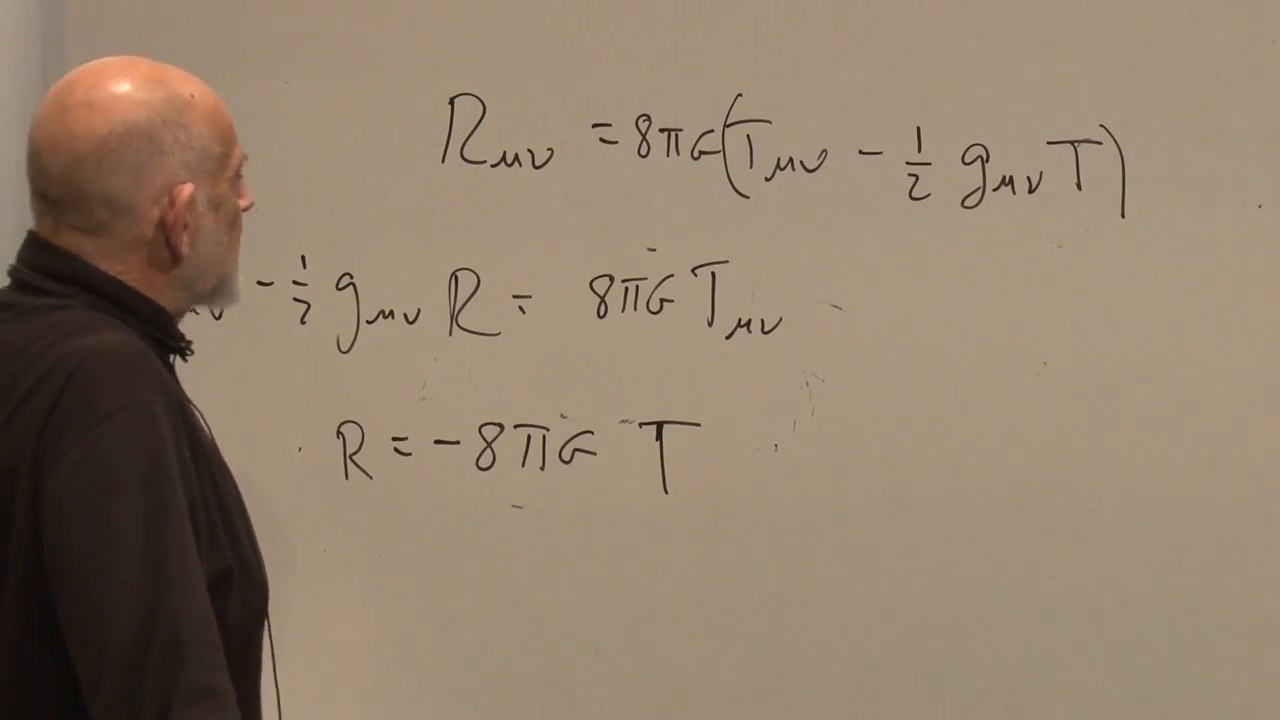
\includegraphics[width=0.82\textwidth]{lecture_09_figure_05.png}
\caption{대각합 관계와 이에 동등한 리치 텐서 형태의 아인슈타인 방정식.}
\lectureframe{01:32:25}
\end{figure}

\begin{classroomqa}
\audiencequestion{스칼라 \(T\)에는 물리적 의미가 있나요?}
\lecturerresponse{이는 에너지-운동량 텐서의 대각합이다. 전자기 복사에서는 이 값이 영이며, 광자처럼 질량이 없는 입자로 이루어진 이상 기체에서도 마찬가지다. 질량을 가진 물질에서는 대개 영이 아니다. 방정식~\eqref{eq:trace-relation}에 따라 이 대각합이 곡률 스칼라를 정한다.
\lecturetimestamp{01:32:20--01:33:12}}
\end{classroomqa}

\section{리치 텐서가 기억하는 곡률의 범위}

\begin{classroomqa}
\audiencequestion{리만 텐서의 작은 폐곡선을 따라 평행이동하는 것에 견줄 만한, 리치 텐서와 리치 스칼라의 간단한 물리적 또는 기하학적 그림이 있나요?}
\lecturerresponse{여기서는 그에 견줄 만큼 명료한 그림을 제시하지 않는다. 리만 텐서는 작은 폐곡선을 따라 평행이동할 때 생기는 회전을 직접 기록한다. 리만 텐서의 축약은 대수적으로 더 간단하지만, 그 각각의 기하학적 의미를 시각화하기는 더 어렵다. 편리하다는 이유만으로 오해를 부르는 그림을 만들어 내지 않는 편이 낫다.
\lecturetimestamp{01:33:14--01:34:13}}
\end{classroomqa}

축약에서 사라지는 정보의 양은 차원에 따라 다르다. 사차원에서 리만 텐서는 리치 텐서에 없는 곡률 정보를 포함한다. 삼차원에서는 리만 텐서가 리치 텐서로 결정된다. 이차원에서는 곡률 스칼라가 독립적인 곡률 정보를 모두 담는다. 따라서 사차원 중력에는 \(R_{\mu\nu}\)에는 드러나지 않는, 원천이 없는 곡률 자유도가 존재할 수 있다.

\begin{classroomqa}
\audiencequestion{서로 다른 리만 텐서가 같은 리치 텐서를 가질 수 있다면, 그 누락된 정보는 물리적으로 어떻게 나타나나요?}
\lecturerresponse{주어진 원천만으로 가능한 모든 중력 배치가 정해지는 것은 아니다. 경계 조건과 초기 조건에는 중력 복사가 포함될 수 있다. 약한 장 근사에서는 원천을 가진 해에서 시작해 자유 중력파를 더한다고 생각할 수 있다. 완전한 비선형 이론에서는 임의의 중첩이 허용되지 않지만, 이 예는 빠진 정보를 올바르게 가리킨다. 즉, \(T_{\mu\nu}\)에 의해 국소적으로 정해지지 않는 전파하는 곡률이다.
\lecturetimestamp{01:37:05--01:38:59}}
\end{classroomqa}

이제 두 가지 진공 사례가 하나로 연결된다. 슈바르츠실트 기하는 질량 바깥에 조석 곡률을 가진다. 중력파는 자유롭게 전파하는 곡률을 가진다. 두 경우 모두 평탄하지 않으면서 \(R_{\mu\nu}=0\)을 만족할 수 있다.

\section{우주 상수}

\begin{classroomqa}
\audiencequestion{우주 상수 같은 추가적인 임의 조정 인자는 없나요?}
\lecturerresponse{우주 상수는 허용된다. 이를 기하학적 좌변에 \(g_{\mu\nu}\)의 상수배로 쓸 수도 있고, 우변으로 옮겨 에너지-운동량 텐서의 진공 기여분으로 해석할 수도 있다. 둘은 계산상 항을 배치하는 방식만 다를 뿐 같은 방정식이다.
\lecturetimestamp{01:39:01--01:40:44}}
\end{classroomqa}

우주 상수를 포함하면 흔히 다음 규약을 쓴다.
\begin{equation}
 G_{\mu\nu}+\Lambda g_{\mu\nu}
 =
 8\pi G\,T_{\mu\nu}.
\end{equation}
추가 항을 우변으로 옮기면 유효 진공 응력 텐서가 정의된다.
\begin{equation}
 T_{\mu\nu}^{(\Lambda)}
 =
 -\frac{\Lambda}{8\pi G}g_{\mu\nu}.
\end{equation}
계량 호환성으로부터 \(D_\mu g^{\mu\nu}=0\)이므로, 추가 항은 자동으로 보존 법칙과 양립한다. 이는 앞서 유일성을 논할 때 열어 두었던 계량 항이다.

\section{수성과 약한 장 계산}

\begin{classroomqa}
\audiencequestion{아인슈타인은 이 방정식으로 수성의 궤도를 계산했나요? 계산 과정은 어디서 볼 수 있나요?}
\lecturerresponse{아인슈타인이 연구할 때는 슈바르츠실트가 정확한 해를 제시하기 전이었다. 아인슈타인은 대신 태양 외부장의 큰 거리 근사로 충분히 정확한 해를 사용했다. 태양의 반지름과 수성의 궤도 크기는 태양의 슈바르츠실트 반지름보다 훨씬 크므로 상대론적 보정은 작다. 케플러 궤도에서 시작해 섭동적으로 보정을 계산할 수 있었다. 얼마 지나지 않아 슈바르츠실트가 정확한 외부 해를 구하면서 같은 계산을 체계적으로 할 수 있게 되었다.
\lecturetimestamp{01:40:46--01:43:48}}
\end{classroomqa}

섭동 이론이란 바로 이런 뜻이다. 이미 풀린 문제에서 시작해 작은 보정의 효과를 계산한다. 뉴턴의 역제곱 힘은 닫힌 케플러 타원 궤도를 만든다. 일반상대성이론은 뉴턴의 반지름 방향 방정식에 작은 변화를 더하므로, 한 바퀴 돈 뒤 타원이 닫히지 않고 근일점이 세차한다.

강의는 닫힌 중심력 궤도가 지닌 흥미로운 특수성에 관한 논의로 마무리된다. 역제곱 힘은 세차 없이 케플러 궤도를 닫히게 하는 특별한 경우다. 더 일반적으로, 베르트랑 정리는 모든 속박 궤도가 닫히는 다른 중심 퍼텐셜로 등방 조화 진동자를 꼽는다. 작은 상대론적 보정은 뉴턴 역학의 이 축퇴성을 없애고, 수성의 세차 운동을 이 장에서 유도한 장방정식의 관측 가능한 징후로 만든다.